\chapter{Link Layer Security: noncoresec} \label{Chp: LLSEC}

802.15.4 Security provides encryption and authentication at Link Layer. In this chapter, we analyse its Contiki implementation, noncoresec.

One thing to be noticed is that IPv6 fragmentation may affect the packet features. However, as most application designers should avoid fragmentation, we assume the packets are not fragmented in this section unless explicitly specified. This effectively means a frame is equivalent to a packet.

Also the term ``broadcast'' in this chapter represents Link Layer broadcast, that is, the frame is broadcasted to all neighbours of sender's.

We always assume the highest Security Level, $7$, is used. At this Security Level, all frames are encrypted and authenticated by AES-128 with CCM* mode, using MIC of 128 bits.

\section{Protocol and Implementation}

\cite{802154sec} analysed some design problems of 802.15.4 Security and  we summarised them in \Cref{Subsec: 802154 Sec Issue}. Since noncoresec supports only network shared key and does not implement ACL, the key management issues are not concerned in our settings. Instead, two potential problems are investigated in this report:

\begin{enumerate}
	\item Nonce reuse
	\item Incompatible anti replay
\end{enumerate}

\subsection{Nonce Reuse}

As we have explained in \Cref{Subsec: 802154 Nonce}, the only variable field in the nonce is Frame Counter. Inspecting the source code, we realised that the Frame Counter is declared as a static variable and therefore is initialised to $0$ on each reboot. This implies that the nonce is reused whenever the device is rebooted.

Our experiments confirmed the vulnerability. We simulated two executions of  broadcast\_example of llsecapps in \Cref{Sec: Applications}, broadcasting the same message. The data shows that frames with identical ciphertext are observed for the same application data with same Frame Counter. In reality, this vulnerability implies that an adversary with capability to reset the device can eventually learn the differences in plaintexts by calculating the differences of ciphertext with the same Frame Counter. This in many cases can cause severe breach of data confidentiality.

One solution might be to store part of the Frame Counter on the flash and increases that value on each reboot, or when the other bits of Frame Counter has reach their maximum. Assuming the device averagely sends one frame every minute, and stores the highest byte of Frame Counter, it will be resilient in $2^8$ reboots and whilst the lower bytes can still has the space of $2^{24}$ frames, which holds up to nearly 32 years. Another solution might be to set the higher bytes of Frame Counter to a random value on each reboot. For example, by setting the highest byte to a uniformly distributed random value in $[0,255]$, the adversary is expected to successfully reset the Frame Counter to a specific value with probability of $2^{-8}$ on each reboot. However, the random approach may be vulnerable to birthday attacks.

The example data is available at: \\
\url{https://github.com/Salties/MyRepository/tree/master/experiments/llsecapps/Data/nonce_reuse}

\subsection{ Incompatible Anti Replay}

\cite{802154sec} has pointed out that anti replay in 802.15.4 Security is incompatible with network key as the same ACL entry is shared among multiple nodes, causing confusion of Replay Counter in ACL. However, after inspecting the source code of noncoresec implementation, we realised that the noncoresec does not suffer from the same problem as ACL is not implemented. Instead, a data structure recording the last Frame Counter of each source address is added to the routing table in kernel to implement the anti replay. Since the last Frame Counter is recorded for each source address, it does not conflict with the network shared key.

\section{AES Timing} \label{Sec: AES Timing}

802.15.4 uses AES-128 for both encryption and authentication as explained in \Cref{Subsec: 802154 Sec}. The noncoresec implementation invokes the AES-128 interface provided by Contiki system library. In Contiki, the underneath AES-128 implementation could be either:
\begin{itemize}
	\item An AES-128 coprocessor on the platform.
	\item A software implementation provided in ``/contiki/core/lib/aes-128.c''.
\end{itemize}

The choice of implementation is controlled by the AES\_128\_CONF macro defined in the platform specific configuration file.

Although CC2538 has an AES coprocessor embedded, but Contiki release-3.0 does not support it. Therefore we examine the following AES implementations those could be used by noncoresec on our platforms:

\begin{enumerate}
	\item AES coprocessor on TelosB.
	\item Contiki software AES on TelosB.
	\item Contiki software AES on CC2538.
\end{enumerate}

We assumed AES to be a pseudo random function and uses its output as random numbers in the experiments.

The AES-128 interface provided by Contiki is as described in \Cref{Contiki AES IF}.

\lstinputlisting[label={Contiki AES IF}, captionpos=b, caption={AES Interface for Contiki release-3.0}]{src/aes_if.c} 

We used the Contiki Real Timer Library\cite{RTimer}, which is a pre-emptive clock library provided by the hardware platform, to measure the system clock ticks of the AES implementations. Each sample measures continuous $n$ rounds executions of AES\_128.encrypt(). 

\Cref{Contiki AES time} shows a simplified code fragment that collects one sample of $n$ round AES execution.

\lstinputlisting[label={Contiki AES time},caption={AES Timing on Contiki release-3.0}, captionpos=b]{src/aes_timing.c} 

\textbf{NEED CALIBRATE!}


We tested this method for  $n \in \{ 50, 100, 150, 200\}$ rounds respectively with random keys and plaintexts. The result is shown in \Cref{Tbl: AES execution time estimation of Contiki}. The measurements are done in system clock ticks. Each round is one AES execution and there are $32768$ ticks per second. We estimate the average time of one AES execution by the slope ratio of rounds and ticks.

\begin{table}[ht!]
	\center
	\begin{tabular}{|c|c|c|c|}
	\hline
	                               & Ticks (TelosB HW) & Ticks (TelosB SW) & Ticks (CC2538 SW) \\ \hline
	50 rounds                      & 633.57                  & 4565.0                  & 981.31                  \\ \hline
	100 rounds                     & 1270.3                  & 9152.58                 & 1947.6                  \\ \hline
	150 rounds                     & 1901.4                  & 13736.13                & 2913.2                  \\ \hline
	200 rounds                     & 2542.4                  & 18298.92                & 3880.0                  \\ \hline
	Correlation(rounds, ticks)     & 1.000                   & 1.000                   & 1.000                   \\ \hline
        Tick per round & 12.72                   & 91.46                   & 19.33                   \\ \hline
	AES Execution Time   & 388.18 us               & 2791.14 us              & 589.90 us               \\ \hline
	\end{tabular}
	\caption{AES execution time estimation on Contiki, with sample size 100}
	\label{Tbl: AES execution time estimation of Contiki}
\end{table}

%Fix vs Random
To verify whether the execution time leaks any information of the AES key, we applied the Fixed vs Random strategy inspired by TVLA\cite{TVLA}, with slight adaptation. To be more specifically, we compared $1000$ samples collected for $n=200$ on fixed and random inputs to the AES implementations respectively, by using t-test\footnote{The timings are assumed to follow a normal, or similar, distribution.} to determine whether a statistical difference can be observed  between two groups. We use the null hypothesis that two groups of AES timing data have the same mean for the t-test. If the null hypothesis is rejected, then we conclude that there is a potential leakage in the timing information as the samples are likely to be distinguishable. 

Theoretically, AES-128 is unlikely to be vulnerable to timing attacks as there is no branch in the algorithm and most of its operations take a constant time; thus the encryption and decryption of a block are expected to be done with a constant time. Even though \cite{Cache-Timing1} and \cite{Cache-Timing2} described attacks that exploits the timing side channel induced by CPU caching, these attacks are unlikely to be replicable on our platforms as the processors do not have cache implemented. 

Nevertheless, our test result surprisingly indicates that there is a potential leakage in the AES execution time on the implementation we tested, as shown in \Cref{Tbl: Fixed vs Random test on Contiki AES timing}.

\begin{table}[ht!]
	\centering
	\begin{tabular}{|c|c|c|c|c|c|}
		\hline
		              & p-value           & $\overline{t}$ for fixed & $s_{T}$ for fixed & $\overline{t}$ for random & $s_{T}$ for random\\ \hline
		TelosB HW AES & $6.08 * 10^{-5}$  & 2536.9     & 4.77      & 2537.7      & 4.38       \\ \hline
		TelosB SW AES & $5.88 * 10^{-14}$ & 18311.9    & 31.54     & 18293.106   & 36.11      \\ \hline
		CC2538 SW AES & 0                 & 3800.49    & 3.93      & 3878.80     & 2.37       \\ \hline
	\end{tabular}
	\caption{Fixed vs Random test result on Contiki AES timing, with $n=200$ and sample size 1000. $\overline{t}$: sample mean of ticks, $s_{T}$: sample standard deviation of ticks.}
	\label{Tbl: Fixed vs Random test on Contiki AES timing}
\end{table}

%Not observable from traffic.
The negligible p-values in \Cref{Tbl: Fixed vs Random test on Contiki AES timing} indicates that there is a statistical significance between the fixed group and random group. However, we have not yet came up with a reasonable explanation of the cause of this variance. We leave this as an open question in this report.

On the other hand, we also noticed that this timing variance is of tens of clock ticks for $200$ executions. In the most significantly variant platform, TelosB Software AES implementation, for one AES execution the timing variance is estimated to be less than $7.63 * 10^{-6}$s based on the sample standard deviation\footnote{Assuming there is no more than $\pm50$ ticks variance for 200 AES executions.}.

Even for a 802.15.4 Frame of MTU size, which is 127 bytes, there is no more than $8$ AES executions for encryption and $8$ executions for MIC computation. Therefore the timing variance is expected to be less than  $1.22 * 10 ^ {-4}$s. Since the bit rate of 802.15.4 PHY is at most 250 kb/s\cite{802154}, i.e. at least $5.08 * 10^{-4}$s is needed to transmit a frame of MTU size in the optimal scenario. Further more, other factors such as RDC and CSMA/CA  may as well induce noises at $10^{-4}$s level, plus the inaccuracy of measurement. We suspect such timing variance on AES execution time would be difficult to observe from the traffic in practice.

%Source code and data
The source code and experiment data are available at:\\
\url{https://github.com/Salties/MyRepository/tree/master/experiments/llsecapps/} \\
and \\
\url{https://github.com/Salties/MyRepository/tree/master/experiments/llsecapps/Data/aestiming}

%\section{Packet Feature Analysis}
%
%In this section, we analyse the general packet features of WSN protected by noncoresec. We focus on the following subjects:
%
%During the experiments, we also realised that the RPL messages can be distinguished in most of our applications by jointly inspect the MAC destination address and frame size, even though it is part of the encrypted MAC Payload.

\section{Frame Size} \label{noncoresec frame size}

As described in \Cref{Subsec: 802154 Sec}, when 802.15.4 Security is enabled, the MAC Frame will have an additional Auxiliary Security Header and MIC. Since no Key Strategy is supported by noncoresec and we imposed Security Level $7$, it is expected that noncoresec will linearly increases the frame size as explained in \Cref{Semantic Packet Size}. To be more specifically, the increment of frame sizes in noncoresec is expected to be $21$ bytes, where $5$ bytes for Auxiliary Header\footnote{Security Level together with Key Strategy are aligned into $1$ byte.} and $16$ bytes for $128$ bits MIC.

%With broadcast and unicast respectively.
Our Cooja simulation confirmed this estimation. We have done two groups of experiments on TelosB mote simulator, one with the broadcast application and the other with unicast application.


\subsection{Broadcast}
In case of broadcast without noncoresec, the relation of application data \footnote{UDP Payload.} size $l_D$ and plaintext MAC Frame size $l_P$ in bytes are:
\begin{equation}
	l_D = l_{P} - 66
\end{equation}

With noncoresec enabled, the application data size $l^{\prime}_D$ and ciphertext MAC Frame size $l_C$ are:
\begin{equation} \label{Eq: broadcast llsec data size}
	l^{\prime}_D = l_{C} - 87
\end{equation}

Assuming the same application data is sent, i.e. $l_D = l^{\prime}_D$, the change of frame size induced by noncoresec is:
\begin{equation}
	b = l_C - l_P = (l^{\prime}_D + 87) - (l_D + 66) = 21
\end{equation}

which is the estimated value.

\subsection{Unicast}

In case of keyllsec unicast application, we have:

\begin{equation}
	l_D= l_P - 80
\end{equation}

\begin{equation} \label{Eq: unicast llsec data size}
	l^{\prime}_D = l_{C} - 101 
\end{equation}

Therefore, 
\begin{equation}
	b = l_C - l_P = (l^{\prime}_D + 87) - (l_D + 66) = 21
\end{equation}

which is exactly the expected value.

\subsection{Conclusion}

In either cases, the size of additional data induced by noncoresec is $21$ bytes. Specifically, \Cref{Eq: broadcast llsec data size} and \Cref{Eq: unicast llsec data size} can be used to deduce the application data size in frames protected by noncoresec.

The example data is available at: \\
\url{https://github.com/Salties/MyRepository/tree/master/experiments/keyllsec/Data/frame_size}


\section{ICMPv6 Messages}

ICMPv6 messages are used in 6LoWPAN for network maintenance. Specifically, RPL messages are a family of ICMPv6 messages those are directly responsible in forming and maintaining a 6LoWPAN network. ICMPv6 messages are solely handled by the Contiki kernel and are thus transparent to upper layer applications. Some of them, including RPL messages, are generated spontaneously by the Contiki kernel even when no application is running. We observed three RPL messages in our experiments, DIS, DIO and DAO. Four ICMPv6 messages are also observed, namely NS, NA and Echo Request/Response. The semantics of these messages are described in \Cref{Subsec: ICMPv6}.

In this section, we analyse their packet features in a noncoresec protected 6LoWPAN network.

\subsection{Packet Size and MAC Destination Address} \label{Size and Dst of ICMP}

In the experiments, we realised that most of the ICMPv6 messages observed have characteristic packet features with respect to packet size and MAC destination address. We summarise their packet features in \Cref{Tbl: Packet Features of ICMPv6 Messages in 6LoWPAN with noncoresec}, where ``0xffff'' is the Link Layer broadcast address.

\begin{table}[ht!]
	\center
	\begin{tabular}{|c|c|c|}
		\hline
		       & Packet Size (bytes) & MAC Destination Address \\ \hline
		DIS    & 85                  & 0xffff                       \\ \hline
		DIO(1.) & 118                 & 0xffff                       \\ \hline
		DIO(1.) & 123                 & unicast                      \\ \hline
		DAO    & 97                  & unicast                      \\ \hline
		NS (1.) & 87                  & 0xffff                       \\ \hline
		NS (1.) & 87                  & unicast                      \\ \hline
		NA     & 87                  & unicast                      \\ \hline
		ECHO(2.)   & $101+x$               & unicast                      \\ \hline
	\end{tabular}
	\caption{Packet Features of ICMPv6 Messages in 6LoWPAN with noncoresec, where 0xffff is the Link Layer broadcast address.}
	\label{Tbl: Packet Features of ICMPv6 Messages in 6LoWPAN with noncoresec}
\end{table}


\paragraph{Explanation of \Cref{Tbl: Packet Features of ICMPv6 Messages in 6LoWPAN with noncoresec}}
\begin{enumerate}
	\item DIO and NS message can be sent in either multicast or unicast. The broadcast DIO message is smaller than the unicast one as it uses an abbreviated IPv6 multicast group address ``ff02::1a''. NS uses another multicast group address, ``ff02::1:ff00:0'', which has the same length as an unicast address. However, both of them are mapped to the same ``0xffff'' Link Layer broadcast address in 802.15.4 MAC Header.
	%ICMP ECHO fragmentation in Wismote network.
	\item The size of ICMP ECHO Request and Response may vary due to its payload. On our host machine which runs on Ubuntu 15.04, the default ping command payload is 56 bytes which is expected to result into a frame of 157 bytes, exceeding the MTU required by 802.15.4 standard\cite{802154} and causes fragmentation. The ``-s'' option is therefore used to reduce the size of ICMP ECHO packets. Theoretically, any packet less than 802.15.4 MTU, i.e. 127 bytes, should not be fragmented; however, in our experiments, we realised that ICMP ECHO packets larger than $107$ bytes, i.e. with payload more than $6$ bytes, will be fragmented. We have not identified the exact reason for the fragmentation but we consider this might be a bug of implementation.
	%No NS and NA in Sky network.
	\item Different ICMPv6 messages maybe observed on different platforms. In our experiments, there is no NS and therefore NA observed in WSN built with TelosB.
\end{enumerate}

%Less than minimum size ICMP.
Recall \Cref{Eq: broadcast llsec data size} and \Cref{Eq: unicast llsec data size}, when at least one byte is sent, the minimum frame sizes are 88 bytes and 102 bytes for broadcast and unicast respectively; therefore packets with size less than these values can be immediately categorised as non application packets, which are effectively ICMPv6 messages in practice. Thus some of the ICMPv6 messages can be distinguished from the application traffic by the packet features, as listed in \Cref{Tbl: Distinguishable ICMP Messages}.

\begin{table}[ht!]
	\centering
	\begin{tabular}{|c|c|}
		\hline
		$<\text{Frame Size}, \text{Destination Address}>$                     & ICMPv6 Message \\ \hline
		\textless85, broadcast\textgreater & DIS            \\ \hline
		\textless87, broadcast\textgreater & NS             \\ \hline
		\textless97, unicast\textgreater   & DAO            \\ \hline
		\textless87, unicast\textgreater   & NS / NA        \\ \hline
	\end{tabular}
	\caption{Distinguishable ICMP Messages}
	\label{Tbl: Distinguishable ICMP Messages}
\end{table}

%NS & NA, DIS & DIO
NA is only sent as a response to NS; therefore if a round trip of two 87 bytes unicast packet is observed, it is likely that the first one is NS and the second NA.  

Other ICMPv6 messages are still possible to be distinguished by \Cref{Tbl: Packet Features of ICMPv6 Messages in 6LoWPAN with noncoresec}, but misidentification may occur if the application happened to send packets of both same size and MAC destination address.

%Full list of ICMP
%Example Data
A list of supported ICMPv6 Messages in Contiki release-3.0 is given in \Cref{Supported ICMPv6}. Some of them not included in \Cref{Tbl: Packet Features of ICMPv6 Messages in 6LoWPAN with noncoresec}, as we did not observe them in our experiments.

The sample data are available at:\\
\url{https://github.com/Salties/MyRepository/tree/master/experiments/llsecapps/Data/ICMPv6}

%CONTINUE FROM HERE
\subsection{ICMPv6 Messages Responding Time}

Exploiting the fact that one could possibly distinguish ICMPv6 messages in the encrypted traffic by packet size and destination MAC addresses as explained in \Cref{Size and Dst of ICMP}, we could possibly  differentiate different hardware by inspecting the response time for the same ICMPv6 message, as different devices have different processing power resulting into different processing time for the same message.

Ideally the most suitable messages to perform this attack would be unicast NS and NA messages, since:
\begin{itemize}
	\item They can always be distinguished from application packets by packet size and MAC destination address, as explained in \Cref{Size and Dst of ICMP}.
	\item NA is immediately sent as a response to unicast NS, allowing precise measurement of the responding time.
\end{itemize}

Unfortunately on our real device platforms, TelosB and CC2538, NS and NA are hardly observable. Alternatively, we measured the response time of ECHO messages, i.e. the interval between an ECHO Request and an ECHO Response, as a proof of concept to this attack.  We show the histograms of the ECHO response time with different setups in \Cref{Fig: Histograms of ECHO response times on different setups}.

\begin{figure*}[ht!]
	\begin{subfigure}{.5\textwidth}
		\centering
		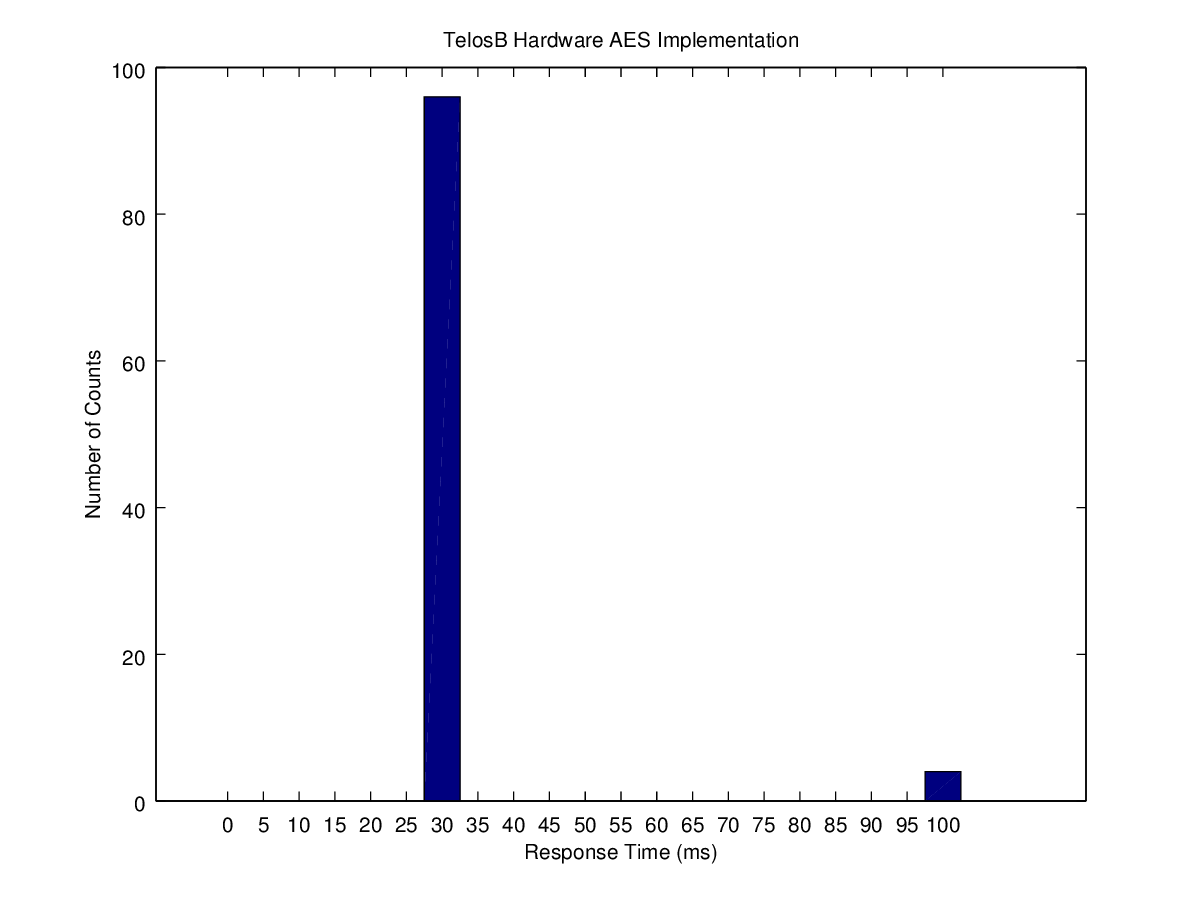
\includegraphics[width=1\linewidth]{fig/noncoresec_ping_telosb_hw.png}
	\end{subfigure}
	\begin{subfigure}{.5\textwidth}
		\centering
		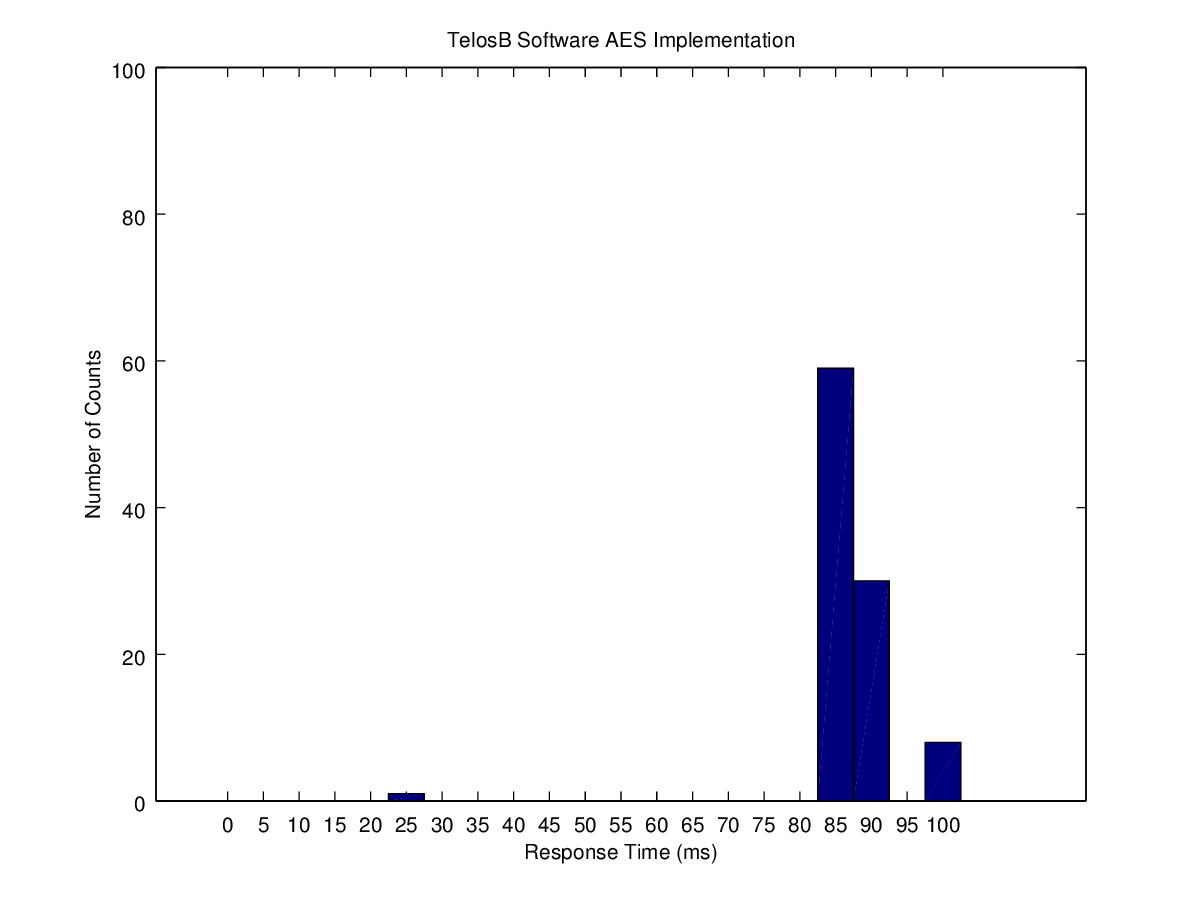
\includegraphics[width=1\linewidth]{fig/noncoresec_ping_telosb_sw.png}
	\end{subfigure}
	\begin{subfigure}{.5\textwidth}
		\centering
		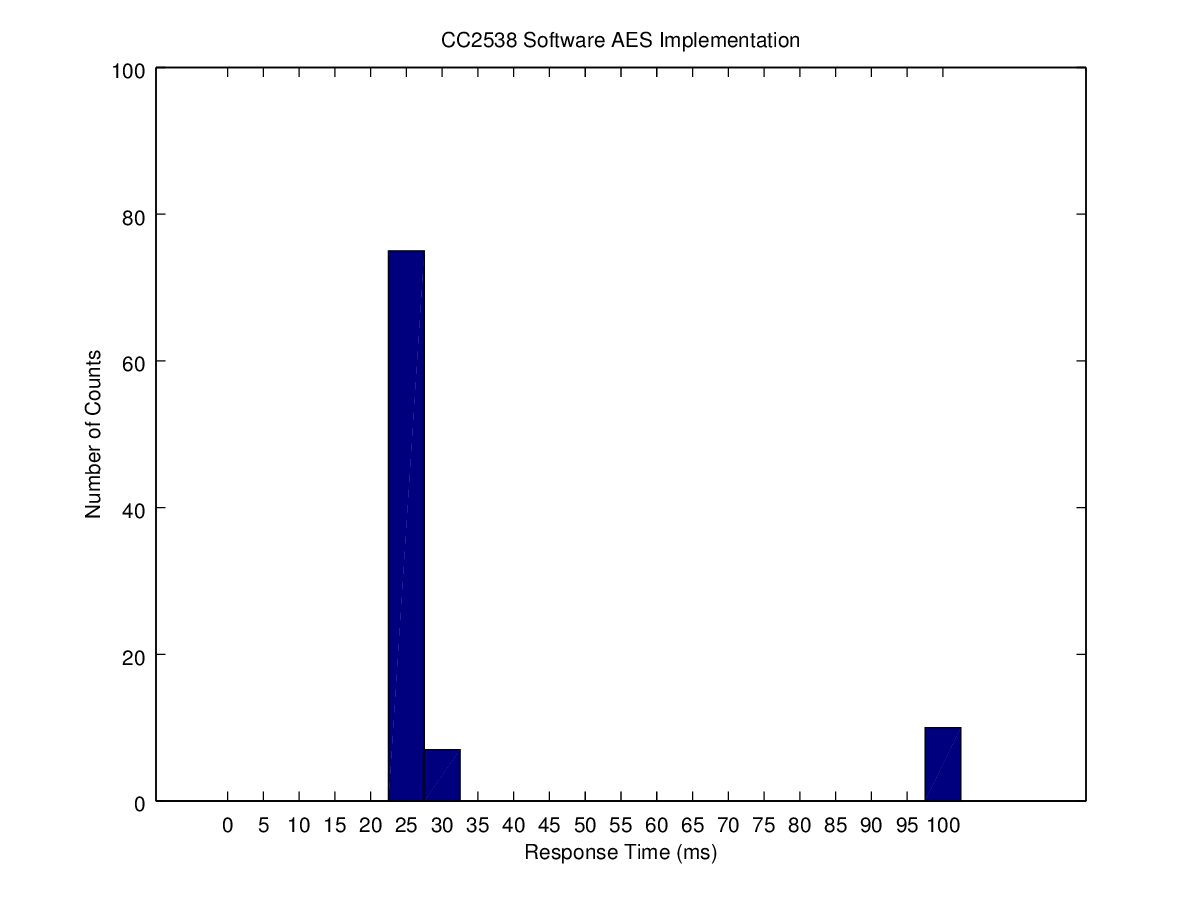
\includegraphics[width=1\linewidth]{fig/noncoresec_ping_cc2538_sw.png}
	\end{subfigure}
	\caption{Histograms of ECHO response times on different setups}
	\label{Fig: Histograms of ECHO response times on different setups}
\end{figure*}

It is obvious that one of the most important character of the distributions shown in \Cref{Fig: Histograms of ECHO response times on different setups} is that the ECHO response times are densely clustered near a specific value in each distribution, while a few of them are ``drifted far away''. Therefore in addition to the means of ECHO response times, we also use their median to characterise their distributions, as summarised in \Cref{Tbl: ECHO Response Time}.

\begin{table}[ht!]
	\center
	\begin{tabular}{|c|c|c|}
		\hline
		              & Mean (ms)     & Median (ms)   \\ \hline
		TelosB HW AES & 37.20 & 30.77 \\ \hline
		TelosB SW AES & 105.19        & 87.4          \\ \hline
		CC2538 SW AES & 48.83         & 24.6          \\ \hline
	\end{tabular}
	\caption{ECHO Response Time}
	\label{Tbl: ECHO Response Time}
\end{table}

We inspect further details of the ``drifted'' values in \Cref{Chp: PINGLOAD}.

The results in \Cref{Tbl: ECHO Response Time} are consistent to our expectations, as CC2538 has much better performance than TelosB even though the hardware AES coprocessor can greatly improve the performance, as shown in \Cref{Tbl: AES execution time estimation of Contiki}.

It is apparent that TelosB with the software AES implementation takes significantly longer time than the other settings. To further verify whether it is distinguishable between CC2538 with software AES implementation and TelosB with hardware AES implementation, we tried the data with two sample t-tests and two sample Kolmogorov-Smirnov tests, KS tests, respectively. For simplicity, we denote $\overline{t}_C$ and $\overline{t}_T$ to be the mean of ECHO response time on CC2538 and TelosB respectively. The test results are shown in \Cref{Tbl: p-values for statistical tests over ECHO response time}.

\begin{table}[ht!]
	\center
	\begin{tabular}{|c|c|c|}
	\hline
	        & $\overline{t}_C == \overline{t}_T$ & $\overline{t}_C < \overline{t}_T$ \\ \hline
	t-test  & 0.146        & 0.927       \\ \hline
	KS test & 0            & 0.567       \\ \hline
	\end{tabular}
	\caption{p-values for statistical tests over ECHO response time. Columns are different null hypothesises.}
	\label{Tbl: p-values for statistical tests over ECHO response time}
\end{table}

The test results suggest that the ECHO response time for CC2538 software AES is likely to be distinguishable from TelosB hardware AES, with CC2538 tends to respond faster than TelosB.

In conclusion, we suggest that the ECHO response time can be potentially exploited to distinguish the platforms and settings in our experiments.

With respect to using the NS/NA messages to perform the same attack, we expect these messages will provide an even better distinguishability as they normally takes longer time to process comparing to ICMP ECHO messages. However, we failed to confirm this due to lack of solutions to generate analysable amount of NS/NA messages on our platforms. We leave this task as a future work in this report.

The data are available at: \\
\url{https://github.com/Salties/MyRepository/tree/master/experiments/llsecapps/ICMPv6/}

\subsection{Countermeasures}

Normally the greatest difficultly of countering these vulnerabilities is the fact that these flaws are built-in nature of the standardised protocol which cannot be easily changed. However, the countermeasures we proposed do not require any modification to the current protocols.

\paragraph{Frame Size}

The most effective and efficient solution to counter the packet size side channel is to pad every packet to MTU. Unlike the similar Traffic Analysis countermeasure on Internet which may cause a drastic overhead, the MTU in a 6LoWPAN network is only 127 bytes which is significantly less than Internet. This effectively means that for those ICMPv6 messages we observed as described in 
\Cref{Tbl: Packet Features of ICMPv6 Messages in 6LoWPAN with noncoresec}, the padding can be no more than $42$ bytes for a single packet. To cope with the current standard, the padding can be done using the Private experimentation type numbers\cite{rfc4443} of ICMPv6, where the receiver can simply silently discard the paddings.

\paragraph{Destination MAC Address}

Due to the nature of RF, all frames are physically broadcasted to all neighbour nodes. As a mitigation to the MAC destination address side channel, the Sensor Nodes may constantly use the Link Layer broadcast address when noncoresec is enabled, and relies on Network Layer to filter out the unintended packets. However, as a consequence, the frames will not be ACKed as ACKs are not sent for broadcast messages and any protocol relies on this feature, such as Contiki MAC, will be affected. We argue this will not cause significant malfunctioning since ACK in 802.15.4 standard is optional and the transmission is always unreliable; therefore any upper layer applications should not rely on  the MAC Layer ACK. However, this method may also cause performance overhead, as those frames supposed to be filtered out at MAC Layer will now be additional passed to Network Layer, resulting into increased computation and power consumption.

\paragraph{Response Time}

Due to the hardware relevance and constrained environment, it would be hard to prevent the timing side channel. One solution might be to treat the responding of ICMPv6 messages as real time tasks, and drop the response if the specified timeout is exceeded. However, dropping the response in some cases may cause excessive performance issue, e.g. triggering flooded retransmissions. In addition, real time tasks are pre emptive, which may result into complicated code that does not fit into the constrained devices. Further more, the pre emptive real time tasks may also induce vulnerabilities to DoS attacks. Alternatively, we may insert dummy operations to randomise the processing time. However, it is unclear whether it is feasible to sample enough randomness without downgrading the functionality of the network. In conclusion, the timing side channel may be hard to mitigate on these platforms.


\section{Conclusion}

In this section we analysed the 802.15.4 Security implementation on Contiki, noncoresec.

noncoresec has a potential nonce reuse problem which can leak the differences of plaintexts by resetting the device.

The execution time of AES implementations on our tested platforms may potentially leak the cryptographic key, but we have not yet identify the cause of the leakage and leave this as an open question. However, this timing leakage is unlikely to be exploitable from the WSN traffic.

Frame sizes has linear relations to the application data, as the number of additional bytes induced by noncoresec is constant.

The ICMPv6 messages are potentially vulnerable targets in a 6LoWPAN network, as they have characteristic packet sizes and MAC destination addresses. Some of them are distinguishable from application packets by the packet features. Further more, the different response time of the same ICMPv6 messages may be exploited to distinguish different hardware in the network. However, countermeasures to the timing side channel are generally difficult to implement in the constrained environment.
